\section{Experiments}
Our generalised shapelet transform, contrasted with the classical shapelet transform, has two extra degrees of freedom: the choice of interpolation scheme $\iota$, and the choice of discrepancy function $\pi^A_S$. In our experiments, we consider $\pi^A_S$ given by either of equations \eqref{eq:learnt-discrepancy} or \eqref{eq:logsignature-discrepancy} and in both cases take the discrepancy parameters $A$ to be diagonal, as this was empirically found empirically to perform best, and the truncation depth of the log-signature is always taken to be $3$. Meanwhile, we take $\iota$ to be piecewise linear interpolation, because efficient algorithms for computing the logsignature transform only exist for piecewise linear paths \cite{signatory}.

For old shapelets, the key hyperparameters to consider are the number of shapelets and the length the these shapelets correspond to. A full description of the hyperparameter selection process is given in Appendix \ref{}. In short we perform a small hyperparameter search for each dataset to optmise the number and length of the shapelets for the old method and use these same parameters in the generalised approach. The length hyperparameter has less meaning in the generalised approach as it is changed during the learning process, but is used in the shapelet initialisation scheme such that the initialised shapelts are the same in all cases.

\subsection{The UEA (Multivariate) Time-Series Archive}
We begin by comparing the classification performance of the old method of shapelets to our new `generalised' approach for which we consider three learnt metrics: a standard L2-metric, an learnt metric and a logsig-3-diagonal. We evaluate the methods on a subset of the UEA time-series archive \cite{bagnall2018uea}. This contains a wide range of multivariate time-series classification problems from various fields with significant differences in time-series length, number of classes, and amount of training data. The full collection contains 30 datasets, however due to algorithm run-time constraints we have considered a subset of these ensuring they still contain significant variation. The statistics of these datasets are given in Table \ref{} of the Appendix.

The results are given in Table \ref{tab:uea_comparison_results}. We see significantly improved classification performance ($> 1$ standard deviation) on $6$ of the $9$ datasets tested with $1$ draw and $2$ losses. We note that the loss on `PenDigits' was extemely close, and the other loss was on `BasicMotions' which has a very small total number samples ($80$) making overfit more likely on the generalised methods (without proper hyperparameter tuning) due to the additional parameters in the model. In contrast, there are many cases where the new method won with significantly higher accuracies than the old method. We also note that the method is sensitive to choice of hyperparameters, and all hyperparameters were chosen for the old method, if hyperparameters were chosen separately for each discrepancy, this would likely improve the results for the learnt discrepancies further.
\begin{table}[ht]
    \centering
    \caption{Classification performance on the UEA datasets from the old shapelet method and the generalised method with a diagonal L2 and diagonal logsig metric with depth 3. The values indicate the classification accuracy on the test set plus or minus one standard deviation. The wins are computed as the number of times each algorithm was within 1 standard deviation from the top score for each dataset.}
    \label{tab:uea_comparison_results}
    \begin{tabular}{lccc}
\toprule
{} & \multicolumn{3}{c}{\textbf{Discrepancy}} \\
\textbf{Dataset} &          L2-diagonal &   logsig-3diagonal &                old \\
\midrule
BasicMotions    &    0.908 $\pm$ 0.014 &  0.808 $\pm$ 0.038 &  0.967 $\pm$ 0.058 \\
ERing           &    0.826 $\pm$ 0.063 &  0.433 $\pm$ 0.029 &  0.672 $\pm$ 0.118 \\
Epilepsy        &    0.884 $\pm$ 0.030 &  0.886 $\pm$ 0.008 &  0.729 $\pm$ 0.054 \\
Handwriting     &    0.103 $\pm$ 0.026 &  0.118 $\pm$ 0.012 &  0.065 $\pm$ 0.037 \\
JapaneseVowels  &    0.972 $\pm$ 0.011 &  0.539 $\pm$ 0.030 &  0.915 $\pm$ 0.041 \\
LSST            &    0.361 $\pm$ 0.002 &  0.357 $\pm$ 0.004 &  0.335 $\pm$ 0.005 \\
Libras          &    0.670 $\pm$ 0.094 &  0.678 $\pm$ 0.055 &  0.622 $\pm$ 0.024 \\
PenDigits       &    0.973 $\pm$ 0.001 &  0.967 $\pm$ 0.007 &  0.975 $\pm$ 0.006 \\
RacketSports    &    0.796 $\pm$ 0.007 &  0.612 $\pm$ 0.092 &  0.796 $\pm$ 0.024 \\ 
\midrule
Wins &            5 &                 3 &    3 \\
\bottomrule
\end{tabular}

\end{table}


\subsubsection{Algorithm Interpretability}
Here we explore the effect of the inclusion of the regularisation term from Equation \cite{eq:interpretable_reg} on shapelet interpretability. Recall that the term was chosen to ensure the resulting shapelets are `close', in the sense of the chosen discrepancy, to some subsample of the training data. To examine this we consider the PenDigits dataset where participants were asked to write down a number from 0-9 and the goal is to classify the intended digit. In Figure \ref{fig:pendigits} we plot, for each digit (0 to 9 in order from left to right), the learnt shapelet that corresponds to the largest coefficient from the logistic-regression for that class. For the old method \ref{fig:old_shapelets}, it is in general not clear what aspect of the digit the shapelet is representing. In some cases the closest digit to the shapelet is not even of the class for which it is thought to best discriminate. Furthermore, the 0 and 1 classes along with the 5 and 8 classes share their `top' shapelet. In contrast, it is abundantly clear what aspect of the digit is being captured by the top shapelets produced from our generalised method \ref{fig:new_shapelets}. Some particular points of interest include shape of the 5 and 6 shapelet being very similar, but the distinction being found in the shapelets chirality (along with its thickness) as the bottom half of a 5 is written clockwise and the 6 anticlockwise. The shapelet for the 7 digit is interesting in its simplicity with it not being immediately clear what makes it so discriminative. By considering those digits with strokes in the top left hand region, we can see that the 8 and 9 have different chiralities to the 7, and the strokes for 1, 2 and 3 are generally written curving upwards to being with wheras 7 is usually flat. A similar such case can be made to explain why the shapelet for the 2 is found to be highly discriminative.

We chose PenDigits here because it is easy to understand visually what the shapelet represents. In general this is not the case, but provided we can make sense of isolated subintervals of the time-series, then the generated results will be interpretable in this context.
\begin{figure}[ht]
    \begin{subfigure}[b]{\linewidth}
        \centering
        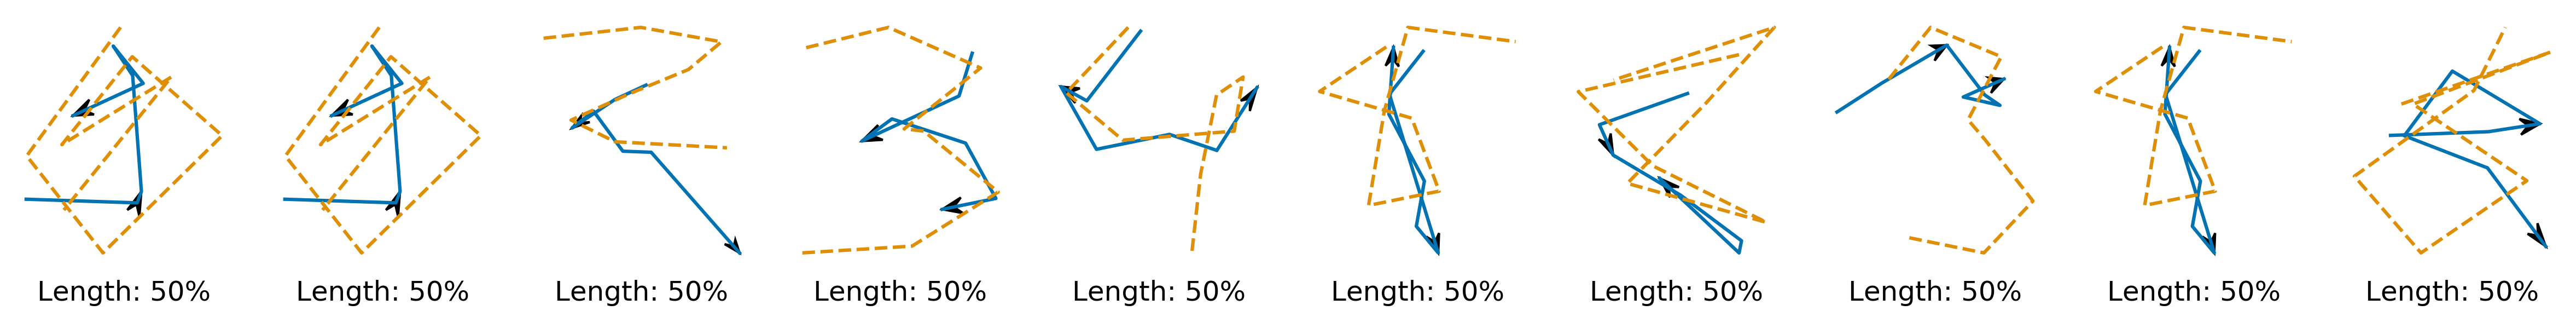
\includegraphics[width=\linewidth]{images/pendigits/old_shapelets_noborder.png}
        \caption{Old shapelets.}
        \label{fig:old_shapelets}
    \end{subfigure}
    \begin{subfigure}[b]{\linewidth}
        \centering
        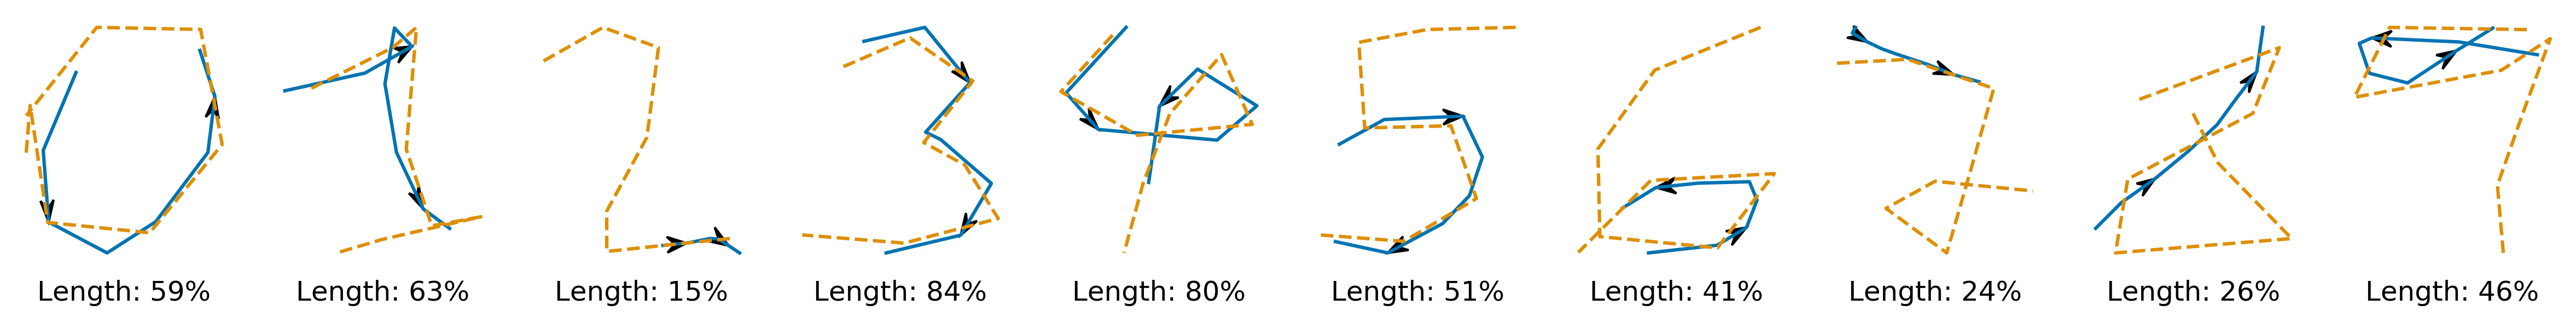
\includegraphics[width=\linewidth]{images/pendigits/new_shapelets_noborder.png}
        \caption{New shapelets.}
        \label{fig:new_shapelets}
    \end{subfigure}
    \caption{The learnt shapelet that corresponds to the largest coefficient in the logistic regression layer for the digits 0 to 9 in order from left to right (blue) and the `closest' path (the path with smallest discrepancy) from the training data (orange dashed).}
    \label{fig:pendigits}
\end{figure}


\subsubsection{Missing Data and Length Ablation}
We now demonstrate both the ability of the proposed framework to handle partially observed data, as well as show the effectiveness of having learnable shapelet lengths.
\begin{table}[ht]
    \caption{}
    \label{tab:uea_noise}
    \centering
    \begin{tabular}{lcccc}
\toprule
{} & \multicolumn{4}{c}{\textbf{Discrepancy}} \\
\textbf{Dataset} &       logsig-3-False &           L2-False &      logsig-3-True &            L2-True \\
\midrule
BasicMotions10    &    0.783 $\pm$ 0.038 &  0.933 $\pm$ 0.038 &  0.767 $\pm$ 0.101 &  0.883 $\pm$ 0.118 \\
BasicMotions30    &    0.825 $\pm$ 0.050 &  0.958 $\pm$ 0.029 &  0.758 $\pm$ 0.063 &  0.942 $\pm$ 0.029 \\
BasicMotions50    &    0.733 $\pm$ 0.115 &  0.942 $\pm$ 0.038 &  0.733 $\pm$ 0.063 &  0.925 $\pm$ 0.066 \\
JapaneseVowels10  &    0.677 $\pm$ 0.082 &  0.955 $\pm$ 0.037 &  0.634 $\pm$ 0.017 &  0.950 $\pm$ 0.034 \\
JapaneseVowels30  &    0.639 $\pm$ 0.025 &  0.968 $\pm$ 0.001 &  0.628 $\pm$ 0.063 &  0.969 $\pm$ 0.002 \\
JapaneseVowels50  &    0.611 $\pm$ 0.061 &  0.968 $\pm$ 0.003 &  0.620 $\pm$ 0.006 &  0.966 $\pm$ 0.003 \\
LSST10            &    0.365 $\pm$ 0.005 &  0.363 $\pm$ 0.001 &  0.359 $\pm$ 0.009 &  0.358 $\pm$ 0.007 \\
LSST30            &    0.360 $\pm$ 0.007 &  0.360 $\pm$ 0.001 &  0.360 $\pm$ 0.007 &  0.407 $\pm$ 0.010 \\
LSST50            &    0.354 $\pm$ 0.007 &  0.362 $\pm$ 0.008 &  0.358 $\pm$ 0.004 &  0.381 $\pm$ 0.034 \\ 
\midrule
Wins &               1 &         5 &              0 &        4 \\
\bottomrule
\end{tabular}

\end{table}


\subsection{Speech Commands}
Finally we examine the performance on the speech commands dataset \ref{warden2018speech} which includes a selection of one-second audio files with each representing a single spoken word. The aim is to build a model to detect the word that has been spoken. We chose this dataset as it is significantly larger than any in the UEA archive so as to demonstrate that the method is not restricted to these (relatively) small datasets. We do reiterate that the computational cost of shapelet methods is high in comparison to other more traditional deep-learning approaches and so can make datasets such as this prohibitive, in particular, it is why we have left the logsig-3 discrepancy out of our analysis in this instance as it takes significantly longer to train compared with the L2 methods.
\begin{table}[ht]
    \caption{Classification accuracy for old shapelets and new shapelets on the Speech Commands dataset.}
    \label{tab:speech_commands}
    \centering
    \begin{tabular}{cc}
\toprule
\multicolumn{2}{c}{Discrepancy} \\
Old &  L2 \\
\midrule
- & - \\
- & - \\
\bottomrule
\end{tabular}

\end{table}

\subsubsection{Interpretability of Speech Commands}
Pray for me.

